% !TEX root = SystemTemplate.tex
\chapter{Design  and Implementation}
The testing program has three main features which needed to be included. These were finding the location of files containing existing test cases for the tested student programs to run, running the single student programs  against the located test cases, and recording and summarizing the test results. C++ was used to write all features.
\\ See Figure~\ref{alg1} below.

\begin{algorithm} [tbh]                     % enter the algorithm environment
\caption{Test C++ Program}          % give the algorithm a caption
\label{alg1}                           % and a label for \ref{} commands later in the document
\begin{algorithmic}                    % enter the algorithmic environment
    \REQUIRE Class directory name from command line
    \ENSURE Test cases are found
    \IF{not in lowest level directory}
        \STATE Find .tst files in current directory
        \STATE Add file paths to .tst file to vector
        \STATE Drop into each subdirectory
    \ELSE
        \STATE Return to parent directory
    \ENDIF
    \ENSURE Test cases are run
    \STATE Compile C++ source code
    \WHILE{not all test cases have been run on all students}
        
        \STATE Run program against next test case
        \STATE Record if test passed/failed or infinite loop
	\STATE Record percentage of code coverage
	\IF{Code profiling enabled}
		\STATE Record code profiling information
	\ENDIF
        
    \ENDWHILE
    \STATE Output .log file with test statistics
\end{algorithmic}
\end{algorithm}
 

\section{Find .spec file, generate cases}
\subsection{Technologies Used}
The technologies used in the component is basic C++.

\subsection{Component Overview}
This component will find a .spec file in any of the directories. If the file exists the user is given the oprion to generate test files to test menus.

\subsection {Phase Overview}
This phase will add .tst files to the directory to test the students source code. 

\subsection {Design Details}
This component finds a .spec file. If it exists, the user will be asked if they want to generate test files to test menus. If the user chooses yes, they will be asked how many files to generate, the max value, and the min value. Then test files are generate so that the values are piped in as input and the student's menu is tested.


\section{Find .tst Files in Subdirectories }

\subsection{Technologies  Used}
The technology used in this component is basic C++.

\subsection{Component  Overview}
This component uses a simple recursive directory crawl to find all .tst files in all subdirectories in the directory passed in via command line. These files will be used to produce output to test student code. 

\subsection{Phase Overview}
This phase will find and queue the .tst files to be used later in testing the students source code.  

\subsection{Architecture  Diagram}
\begin{figure}[H]
\begin{center}
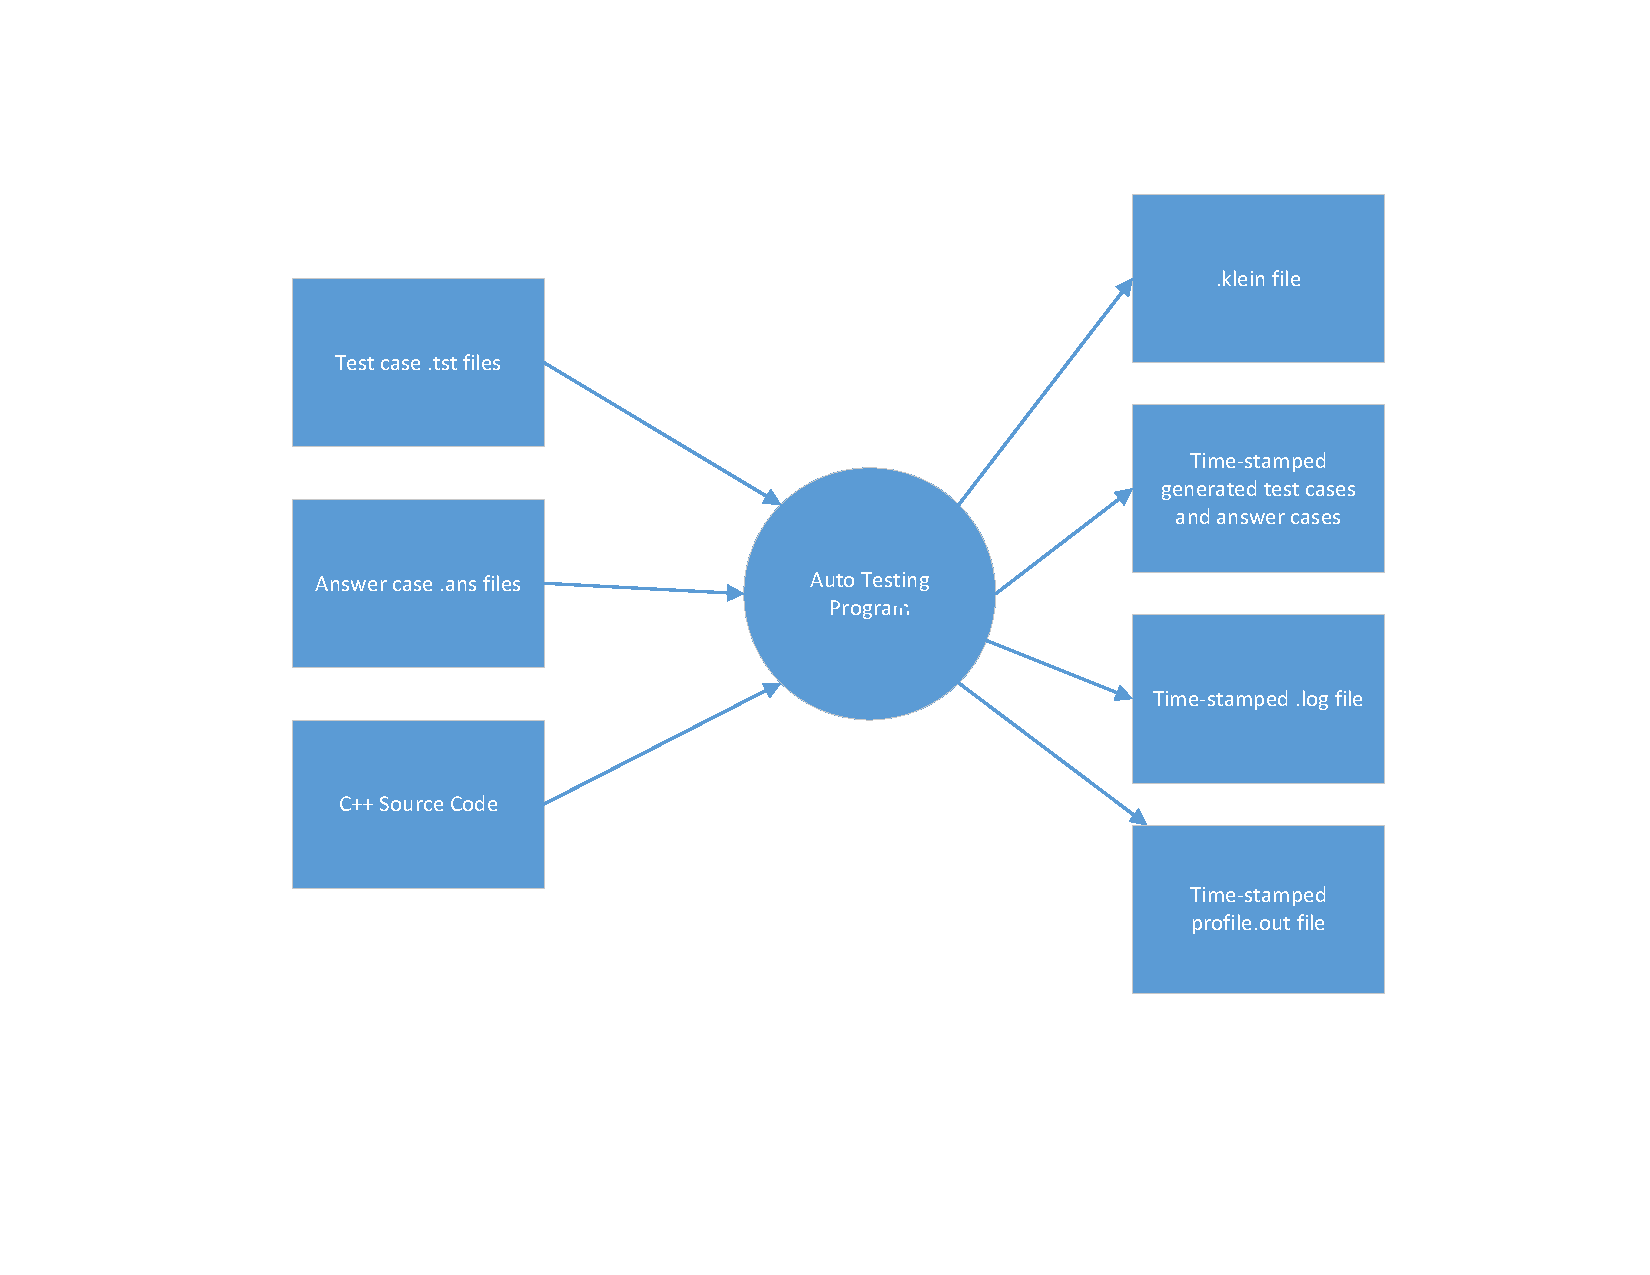
\includegraphics[width=0.75\textwidth]{./ArchitectDiagram}
\end{center}
\caption{Architecture Diagram for the Tester Application \label{arch_generic}}
\end{figure}


\subsection{Data Flow Diagram} 
%See Figure~\ref{dataflow}.



\begin{figure}[H]
\begin{center}
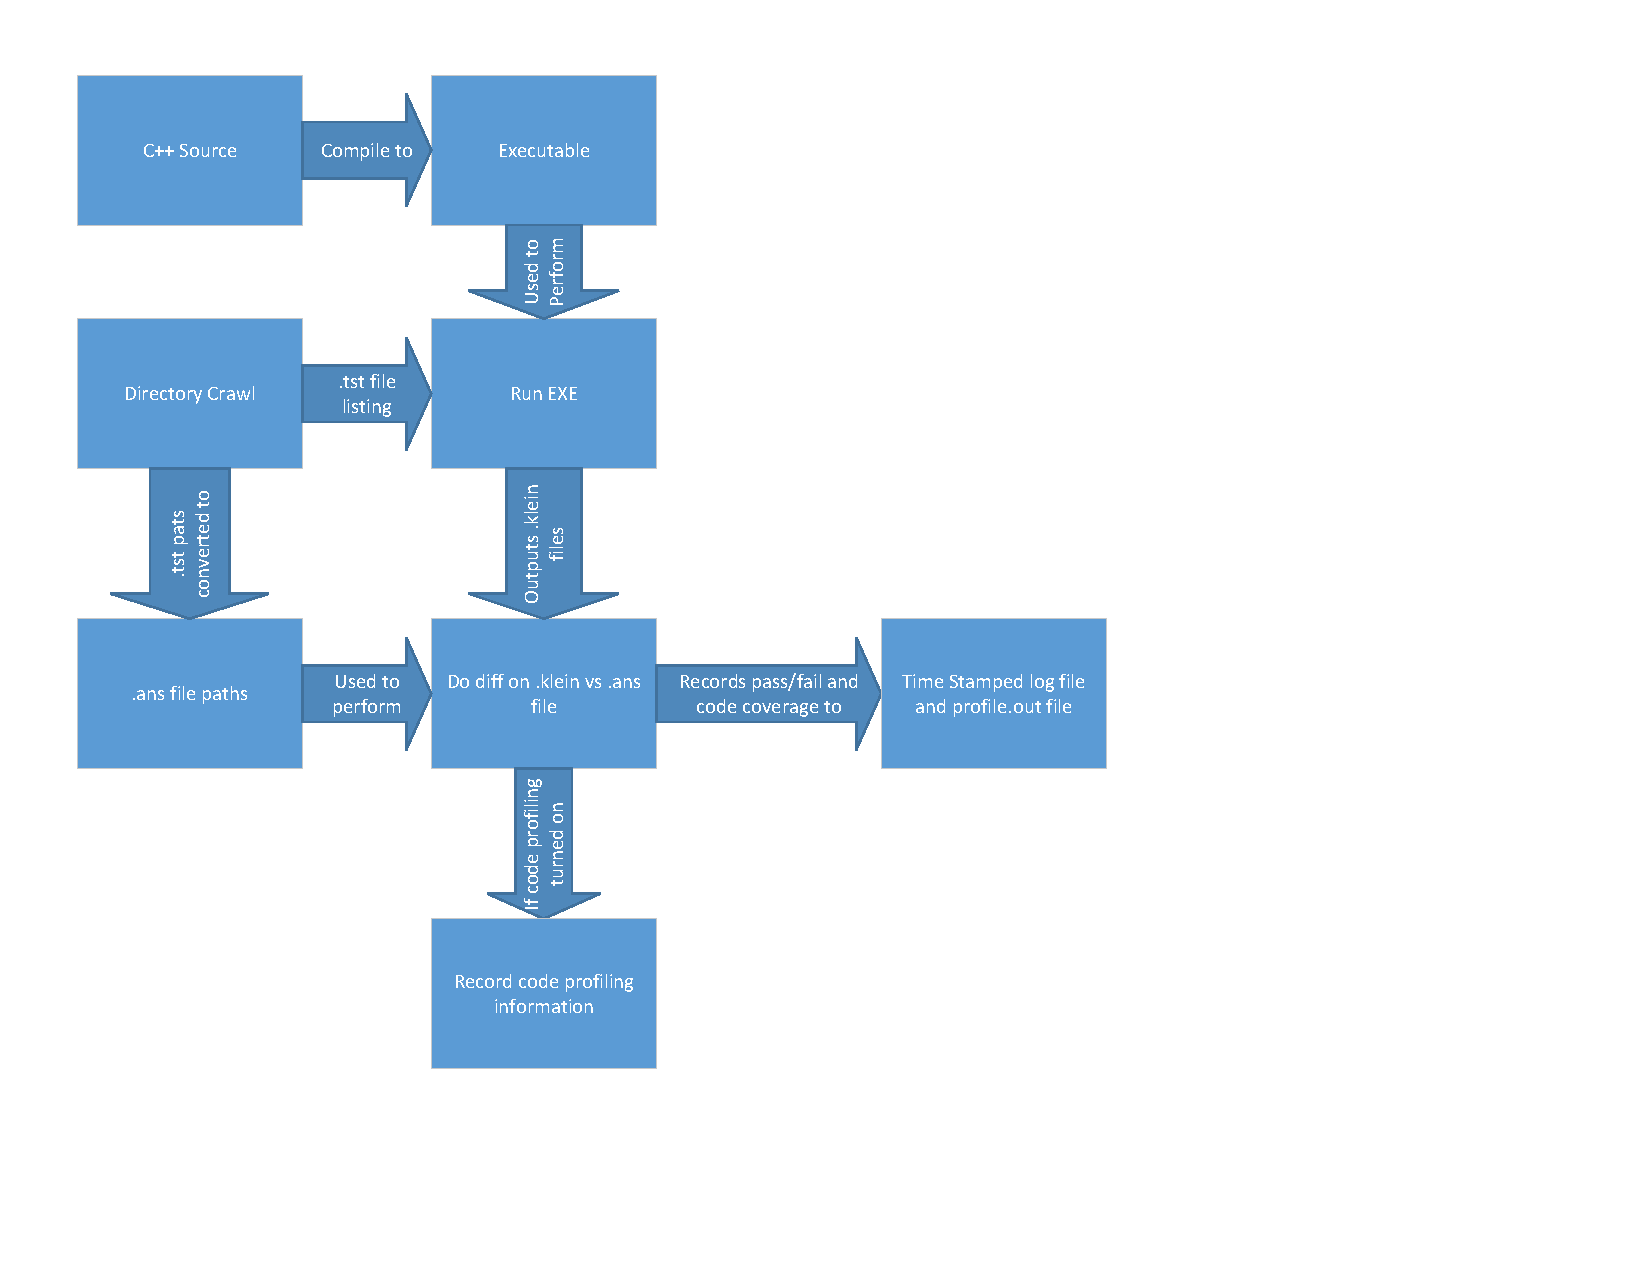
\includegraphics[width=1.45\textwidth]{./dataflow}
\end{center}
\caption{ Data Flow Diagram for the Tester Application \label{dataflow}}
\end{figure}


\subsection{Design Details}
The following function does the directory crawl and stores the relative path to 
 .tst file in the "dest" vector which is passed by reference. This is the recursive function that searches all sub-directories of the directory root which contains the executable program:
\begin{lstlisting}
// Recursive Directory Crawl
void TestSuite::dirCrawl(string targetExt, string dir, vector<string> &dest)
{
    // Open current directory.
    DIR * proc = opendir( dir.c_str() );

    if (NULL == proc)
    {
        return;
    }

    // Read current directory.
    dirent * entry = readdir(proc);

    do
    {
        // Make recursive calls to sub directories
        if(DT_DIR == entry->d_type)
        {
            string name = entry->d_name;
            if ( "." != name && ".." != name )
            {
                string newDir = dir + "/" + entry->d_name;
                dirCrawl( targetExt, newDir, dest );
            }
        }
        // Watch for files with .tst extension
        else if ( DT_REG == entry->d_type )
        {
            string fileName = entry->d_name;
            unsigned int extPos = fileName.rfind(".");
            if ( extPos != string::npos )
            {
                string ext = fileName.substr( extPos );
                if ( ".tst" == ext )
                {
                    fileName = dir + "/" + fileName;
                    cout << fileName << endl;
                    dest.push_back(fileName);
                }
            }
        }
    }while(entry=readdir(proc));

    closedir(proc);
}
\end{lstlisting}
Once this function has finished executing the destination vector contains a listing of all paths to .tst files to be run by the program being tested.



\section{Test Single Program Against Found Test Cases}

\subsection{Technologies  Used}
The only technology used in this section is C++ code.

\subsection{Component  Overview}
The purpose for this section is to compile the C++ code, loop through the list of .tst files in the directory, and check if the program output matches the .ans file output.

\subsection{Phase Overview}
Testing a program against located test cases is necessary in the second and third phases because we must be able to check the program's output against the .ans file to see if each test was a success or failure before program output can be prepared.

\subsection{ Architecture  Diagram}
Due to the small size of the application, a single diagram describing the architecture of the program is provided in Figure~\ref{arch_generic}

\subsection{Data Flow Diagram}
Due to the small size of the application, a single diagram describing the data flow for the program is provided in Figure~\ref{dataflow}.


\subsection{Design Details}
Testing the program may be broken down into three sections:
\begin{itemize}
	\item Compiling source C++ code
	\item Running C++ code against test case
	\item Determining if program output was correct for test case
\end{itemize}
The following function compiles the program using a system call to g++:
\begin{lstlisting}
//Function to compile c++ source code based on filename
bool TestSuite::compile_code( string filename )
{   string compile_instruction = "g++ "; // Form the string for the system call
    compile_instruction += filename;
    compile_instruction += " -o test_prog";

    system( compile_instruction.c_str() );

    return true;
}\end{lstlisting}
To run the executable against a test case another system call is made redirecting input from the test file and output to the ".klein" file:
\begin{lstlisting}
//Function to run c++ souce with redirected input/output
bool TestSuite::run_code( string test_file )
{   string run_instruction = "./test_prog < ";  //Form the string for the system call
    run_instruction += test_file;
    run_instruction += " > test_out.klein";

    system( run_instruction.c_str() );

    return true;
}
\end{lstlisting}
Finally, the program output file needs to be compared to the .ans file. This is also done with a system call to diff:
\begin{lstlisting}
//Function to do diff on answer file and test program output file
bool TestSuite::correct_answer( string ans_file )
{  string diff_instruction = "diff test_out.klein ";
    diff_instruction += ans_file;
 
   return (! system( diff_instruction.c_str() ) );
}
\end{lstlisting}
The only change to compare all the test files is to place the preceding functions in a loop and pass each new test file as a parameter to run\_code() which is done in run\_test() as follows:
\begin{lstlisting}
// Runs program with input from test files in testFiles vector.
void TestSuite::runTests()
{  numCorrect = numWrong = 0;
    pair<string, bool> result;

    vector<string>::iterator it;           // Iterate over test files.
    for ( it = testFiles.begin(); it != testFiles.end() ; it++ )
    {
        // Run program with given test file.
        run_code(*it);

        // Determine corresponding answer file.
        string ans = *it;
        ans.replace(ans.end()-4, ans.end(),answerExtension);

        // Populate results vector and counters.
        result.first = *it;
        if (correct_answer(ans))
        {
            result.second = true;
            numCorrect++;
        }
        else
        {
            result.second = false;
            numWrong++;
        }
        // Add results to vector.
        results.push_back(result);
    }
}
\end{lstlisting}
Upon completion, the TestSuite object contains counters for the number of correct and incorrect test cases to be used when outputting the log file.

\section{Record and Summarize Test Results }

\subsection{Technologies  Used}
The only technology used in this section is C++ code.

\subsection{Component  Overview}
After the test cases have been run a timestamped .log file needs to be produced. It should include if each test case passed or failed as well as the percentage of correct files along with the total number of correct and incorrect test cases.

\subsection{Phase Overview}
This component is included in the fourth phase of production. It was done last because the full output file could not be produced without knowing the results of all the test cases.

\subsection{ Architecture  Diagram}
Due to the small size of the application, a single diagram describing the architecture of the program is provided in Figure~\ref{arch_generic}


\subsection{Data Flow Diagram}
Due to the small size of the application, a single diagram describing the data flow for the program is provided in Figure~\ref{dataflow}.

\subsection{Design Details}
The formatted output is produced by the outputLogFile() function. It lists if each test case was a pass or failure along with overall test statistics. In each student directory a gcov and gprof file will be generate to analyze performance and code coverage. 


